\appendix
\chapter{Helpful Things}
\section{LP formulations}
\subsection{Maximum Flow}
Note: this proves LP solving is P-complete.

We want to maximise the flow between a source $s$ and a sink $t$ in a directed graph with edge capacities $c_e, e\in E$.

\begin{align*}
\max \quad & \sum_{e\in O(s)} f_e\\
\intertext{Flow conservation: $I$ for incoming edges, $O$ for outgoing edges}
s.t.\quad	& \sum_{e\in I(v)} f_e - \sum_{e\in O(v)} f_e = 0 && \forall v\in V\backslash {s,t}\\
\intertext{Capacities:}
	& f_e \leq c_e && \forall e \in E\\
\end{align*}

It's easy to generalise to an arbitrary number of sources/sinks by introducing supply/demand variables $b_v$ for all $v\in V$ and adding them to the RHS of the flow conservation. The dual of this program computes the minimum cut in the graph.

\subsection{Shortest Paths}

We have a directed graph with weighted edges and no negative weight cycles. We want to solve a single source shortest paths problem. The LP will compute the distances from a node $s$ to all other nodes.

This one is a bit counterintuitive, instead of minimising lengths, we maximise distances

\begin{align*}
\max \quad & \sum_{v\in V} d_v\\
s.t. \quad & d_u \leq c_{uv} + d_v && \forall (u,v) \in E
\end{align*}

With $d_s$ fixed to 0. 

Think about why minimising won't work. Hint: look at the two nodes case.

\subsection{Maximum Matching}

See section \ref{sec:maxAssignment}. We have a bipartite graph $G=(U\cup V,E)$ and want to find a maximum weight perfect matching.

\begin{align*}
\max \quad &  \sum_{i,j} x_{ij} c(i,j)\\
\intertext{everyone in $V$ has one partner}
s.t. & \sum_{i\in U} x_{ij}=1 && \forall j\in V \\
\intertext{everyone in $U$ has one partner}
&\sum_{j\in V} x_{ij} = 1 && \forall i\in U\\
&x_{ij}\in \{0,1\}
\end{align*}

Since this LP is integral (the constraint matrix is the adjacency matrix of a bipartite graph and hence totally unimodular), it is save to drop the integrality constraints.

\subsection{Minimum Spanning Tree}

We have a undirected graph with integral edge weights and want to find a spanning tree of minimum weight.

\begin{align*}
\min \quad &\sum_e c_e x_e\\
\intertext{Build a tree:}
s.t. \quad & \sum_e x_e = |V| -1 \\
\intertext{Subtour elimination:}
	& \sum_{e\in S} x_e \leq |S| -1 && \forall S \subset V
\end{align*}

It is not immediately clear that this works without restricting $x_e\in \{0,1\}$. However this system is TDI and the RHS is integral, hence the polyhedron is integral.

To see why have a look at the dual system:

\begin{align*}
\max \quad & (|V|-1)y_1 + \sum_{S\subset V} (|S|-1)y_S\\
s.t. \quad & y_1 + \sum_{S\ni e} y_S \leq c_e && \forall e\in E\\ 
	& y_1 \text{ free}\\
	& y_S \leq 0
\end{align*}

We can greedily construct an optimal solution for the dual system by following Kruskal's algorithm. Suppose the edges are ordered ascending by weight $c(e_1)\leq c(e_2)\leq \ldots \leq c(e_m)$. 

Let $E_i$ denote the edge set that is selected at step $i$ in Kruskal's algorithm, i.e. the first $i$ edges, and let $S_i$ be the set of corresponding nodes. Since we discard edges that form cycles it is possible that $S_i=S_j, i<j$. Define $e(S_i)$ to be the last edge added to $S_i$ and let $f(S_i)$ be the first edge that will be added to the MST that leaves $S_i$, i.e. the edge that fuses that connected component with another. $f(V)$ is undefined, $e(V)$ is the last edge added to the MST by Kruskal's algorithm.

With this notation we can set the dual variables as follows:

\begin{align*}
y_S^* &= \begin{cases}
c(e(S)) - c(f(S)) & \exists i: S=S_i, S\neq V\\
-c(e(V)) 	& S=V, c(e(V)) \geq 0\\
0	& \text{otherwise}\end{cases}\\
y_1^* &= \begin{cases}
0 & c(e(V)) \geq 0\\
c(e(V)) & \text{otherwise}
\end{cases}
\end{align*}

Clearly these values are integers. They are also $\leq 0$, since $c(e(S)) \leq c(f(S))$ because the edge $f(S)$ is added later. The argument that they satisfy the constraints is a bit complicated:

Consider an arbitrary edge $e_i$. We can rewrite the constraint like this:

\[-\sum_{S\ni e} y_S^* \geq -c_e + y_1^*\]

Assume $c(e(V))\geq 0$ (the other case works similarly). Then $y_1^*=0$ and $y_V^*=-c(e(V)$. Consider the sequence of growing node sets that contain $e_i$ as they are constructed by the algorithm:

\begin{align*}
U_1 &\equiv S_i\\
U_2 &\equiv S_i \cup f(S_i)\\
&\vdots\\
U_l &\equiv V
\end{align*}

Using these nodesets we observe

\[\sum_{S\ni e} y_S^* = \sum_{j=1}^l y_{U_j}^*\]

because for any $S\neq U_j$ for any $j$ either $S$ does not contain both endpoint of $e_i$ or $S$ is not part of the $S_i$. Now the inequality follows because most terms in that sum cancel out as $f(U_i)=e(U_{i+1})$

\begin{align*}
-\sum_{j=1}^l y_{U_j}^* &= -(c(e(U_1)) - c(f(U_1))) - (c(e(U_2)) - c(f(U_2)) - \ldots + (-c(e(V)))\\
	&=-c(e(U_1)) \geq -c_e
\end{align*}

We need to show that this is an optimal solution by using the complementary slackness conditions. Recall from theorem \ref{thm:complSlackness}, solutions $x,y$ are optimal iff

\begin{align*}
y_i(a_ix-b_i) = 0 && \forall i\\ 
(c_j - \trans yA_j)x_j =0 && \forall j
\end{align*}

For $x$ we use the MST we constructed during Kruskal's algorithm. The first equality holds because either $y_S^*$ is 0 or there are exactly $|S_i|-1$ edges in the MST that are contained in $S_i$. The second equality holds because we have for every edge $e_i$ in the tree that $c(e(S_i))=c(e_i)$.

Thus the dual has integral optimal solutions of the same value as the primal (by strong duality) for any integral cost vector $c$, hence the TDIness is proven and it is save to remove the integrality constraints.


\section{ILP formulations}

\subsection{Satisfiability}
See section \ref{sec:ilpNPcomplete}. Note: this proves ILP solving is NP-complete. It may be worthwhile to remember the proof why Satisfiability is NP-complete and use it to cheat your way around exam questions. If you can remember the name of a non-LP algorithm for the problem you are asked to solve copy down the proof, argue that \$Problem is in NP and write down this ILP:

For each variable $v_j$ in the formula we introduce $z_j \in \{0,1\}$ in our ILP, with the natural interpretation of the value of $z_j$. For every clause $C_i$ let $J^+_i$ be the number of positive and $J^-_i$ be the number of negated variables in clause $C_i$.

The ILP for the formula is then

\begin{align*}
\max \quad & 42 \\
s.t. &\sum_{j\in J^+_i} z_j + \sum_{j\in J^-_i} (1-z_j) \geq 1 && \forall i\\
&z_j \in \{0,1\}
\end{align*}

\subsection{Travelling Salesman}

We have a complete graph with weighted edges and want to find a tour of minimal weight.

\begin{align*}
\min \quad & \sum_e c_e x_e\\
\intertext{form a tour}
s.t. \quad & \sum_{e\in \delta(v)} x_e = 2 && \forall v\\
\intertext{subtour elimination}
	& \sum_e x_e \leq |S|-1 && \forall S \subsetneq V, |S|\geq 2\\ 
	& x_e \in \{0,1\}
\end{align*}

\subsection{Knapsack}

The usual knapsack problem involves a set of items with weight and profit. We want to maximise the profit while staying under a maximum weight $K$. This is possibly the easiest ILP of them all:

\begin{align*}
\max \quad & \sum_i p_ix_i\\
s.t.\quad & \sum_i w_i x_i \leq K\\
	& x_i\in \{0,1\}
\end{align*}

\subsection{Maximum Clique}

What size is the maximum clique in a given graph? Let $x_i$ be a variable that tells whether a vertex $i$ is in the maximum clique or not. Via the definition that a clique is a set of vertices no two of which are nonadjacent, the size of a maximum clique is
\begin{align*}
\max \quad & \sum_{i=1}^n x_i\\
\text{s.\,t.} \quad & x_i + x_j \leq 1 & \forall (i,j) \notin E\\
& x_i \in \{0,1\}
\end{align*}

\subsection{Facility Placement}

A special kind of bipartite matching problem where we want to serve customers $i\in [n]$ using facilities $j\in [m]$. There is an edge $e_{ij}$ if customer $i$ can be satisfied by facility $j$. Satisfying a customer yields a profit $p_i$, opening a facility costs $c_j$.

\begin{align*}
\max \quad & \sum_i p_i x_ij - \sum_{j} c_j y_j\\
\intertext{open facility if customers are served by it}
s.t. \quad & \sum_{i} x_{ij} \leq n\cdot y_j\\
	& x_{ij},y_j \in \{0,1\}
\end{align*}

\subsection{Sequencing with Setup Times}

We have a machine that can perform $m$ different operations. Each operation needs a different tool. The machine can hold $B$ tools in its tool magazine. Changing a tool incurs a setup time $s_j$. We need to perform a set of tasks, but we can switch the order. What is the order that minimises the total time?

Introduce $x_{ir}$ that indicates whether job $i$ is performed in slot $r$. $y_{jr}$ means we have tool $j$ in the toolbox at slot $r$.

\begin{align*}
\intertext{Costs only happen when we switch tools}
\min \quad & \sum_r\sum_j s_j|y_{jr}-y_{j(r-1)}|\\
\intertext{we can't hold infinitely many tools in our toolbox}
s.t.\quad	& \sum_j y_{jr} \leq B && \forall r\\
\intertext{we need some tool to complete a job}
	& x_{ir} \leq y_{ir} && \text{easily extended to sets of tools}\\
\intertext{One job at a time}
	& \sum_i x_{ir} = 1 && \forall r
	& x,y\in \{0,1\}
\end{align*}

The absolute value in the objective function can easily be replaced by some new variables $z_{jr}$

\[z_{jr} \geq y_{jr} - y_{j(r-1)} \qquad z_{jr} \geq y_{j(r-1)} - y_{jr}\]

\subsection{Covering and Packing Problems}
\subsubsection{Overview}
\begin{figure}[htbp]
\begin{center}
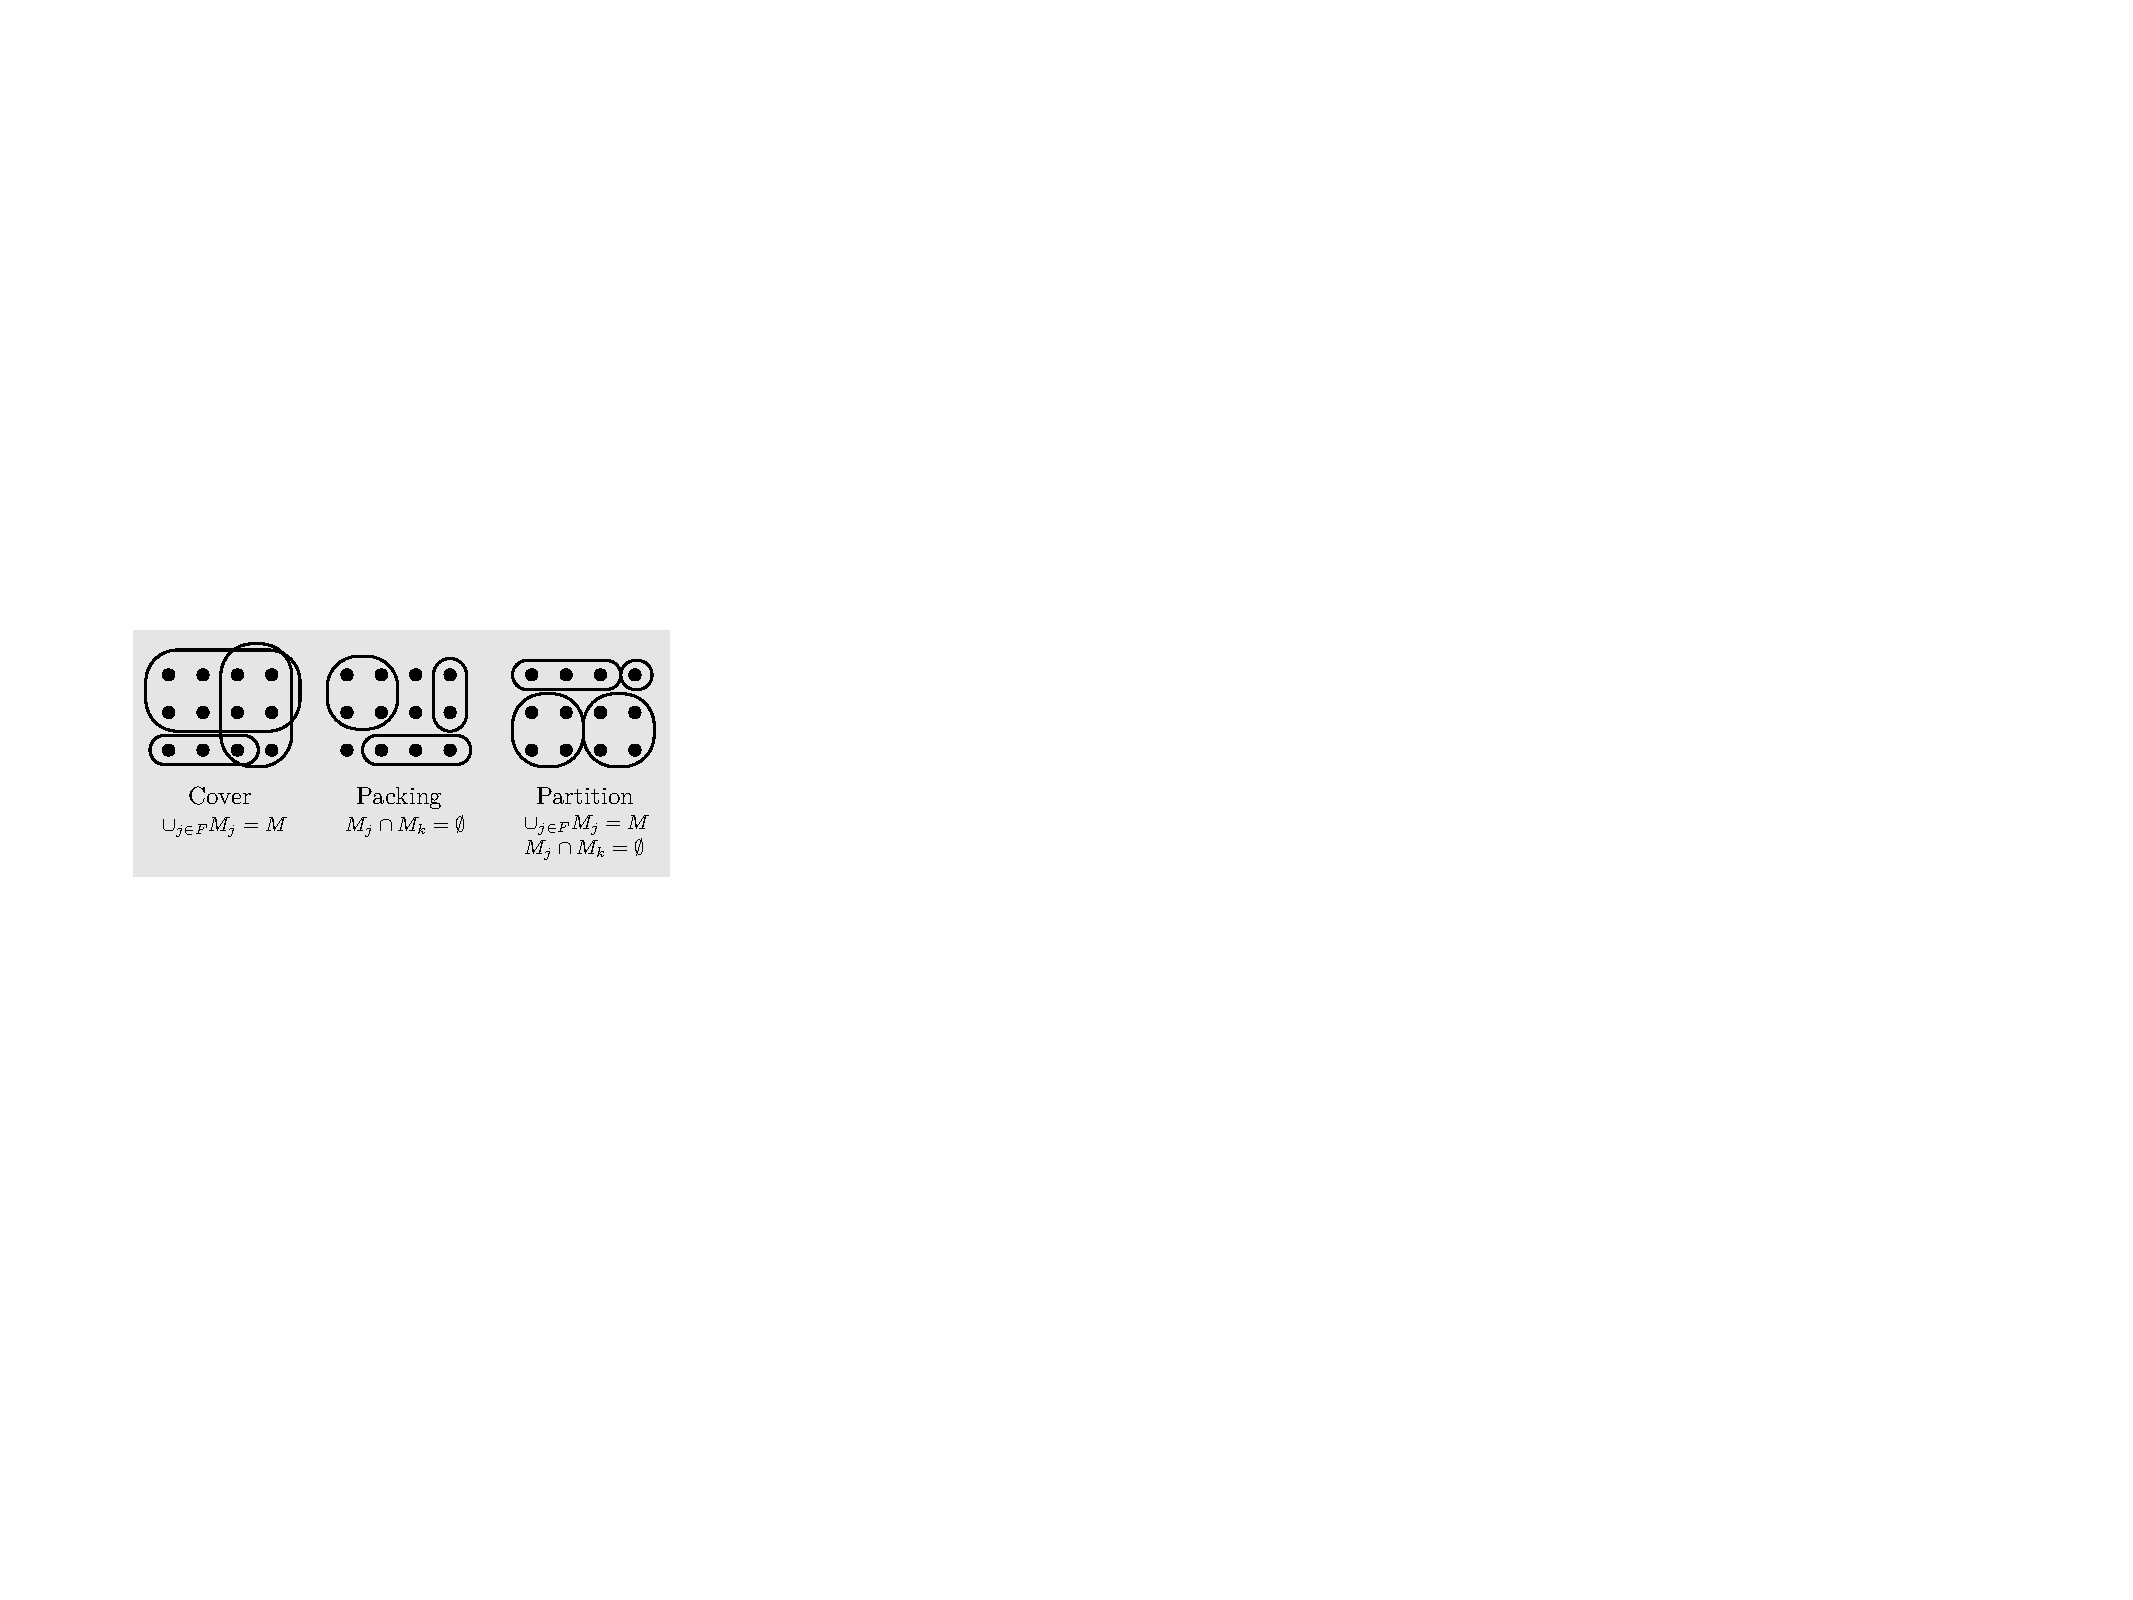
\includegraphics{images/coverpackingpartition}
\caption{Illustration of a cover, a packing and a partition}
\label{fig:coverpackingpartition}
\end{center}
\end{figure}

Let $M = \{1, \ldots, m\}$ and $N=\{1, \ldots, n\}$. Let $M_1, M_2, \ldots, M_n$ be a given collection of subsets of $M$. We are also given a weight $c_j$ for each set $M_j$ in the collection. The weight of a subset $F$ of $N$ is defined as $\sum_{j \in F}c_j$. No we can differentiate between the following set types (cp. figure \ref{fig:coverpackingpartition}):

\begin{itemize}
	\item{A subset $F$ of $N$ is a \emph{cover} of $M$ if $\cup_{j \in F}M_j = M$. In the \textbf{set covering problem} we would like to find a cover F of \emph{minimum} weight.}
	\item{A subset $F$ is a \emph{packing} of $M$ if $M_j \cap M_k$ is empty for all $j,k \in F, j \neq k$. In the \textbf{set packing problem} we would like to find a packing $F$ of \emph{maximum} weight.}
	\item{A subset $F$ is a \emph{partition} of $M$ if it is both a cover and a packing of $M$. In the \textbf{set partitioning problem} both minimization and maximization versions are possible.}
\end{itemize}

\subsubsection{Dualities}
We can observe the following primal-dual relations:

\begin{center}
\begin{tabular}{c|c}
\textbf{Covering problems} & \textbf{Packing problems}\\
\hline
Minimum set cover &	Maximum set packing\\
Minimum vertex cover & Maximum matching\\
Minimum edge cover & Maximum independent set\\
\end{tabular}
\end{center}

\subsection{Covering Problems}

Weighted versions can easily be derived.

\subsubsection{Minimum Set Cover}

We have a set of not necessarily disjoint sets $S=S_i$ from a universe $\mathcal{U}$ and want to find a minimal set of items $u_i$ s.t. each $S_i$ contains at least one of them.

\begin{align*}
\min \quad & \sum_i x_{u_i}\\
s.t. \quad & \sum_{u\in S_i} x_{u} \geq 1 && \forall i\\
	& x_{u_i} \in \{0,1\}
\end{align*}

\subsubsection{Minimum Vertex Cover}

This is a special case of set cover. We want to select a minimal set of edges in a graph s.t. each node is covered by at least one edge.

\begin{align*}
\min \quad & \sum_e x_e \\
s.t. \quad & \sum_{e\in \delta(v)} x_e \geq 1 && \forall v\\
	& x_{e} \in \{0,1\}
\end{align*}
\subsubsection{Minimum Edge Cover}

Same thing again, this time we want to select vertices s.t. all edges are covered.

\begin{align*}
\min \quad & \sum_v x_v \\
s.t. \quad & x_u+x_v \geq 1 && \forall (u,v) \in E\\
	& x_v \in \{0,1\}
\end{align*}

\subsection{Packing Problems}

Weighted versions can easily be derived.

\subsubsection{Maximum set packing}
We want to find a maximal number of disjoint sets in a set of sets.

\begin{align*}
\max \quad & \sum_{i} x_i\\
s.t. \quad & \sum_{i\in S} x_i \leq 1\\
	& x_i \in \{0,1\}
\end{align*}
\subsubsection{Maximum independent set}

Again a special case of maximum set packing, but in graphs. We want to find a maximal set of nodes that is not connected by edges.

Careful: I at least always get this confused with the \emph{maximal} independent set, which can be easily found by a greedy algorithm.
\subsection{Set Partitioning}
This is the combination of a packing and a covering problem. Just replace the $\leq$ or $\geq$ with equality.